\documentclass[12pt,a4]{article}
\usepackage{physics, amsmath,amsfonts,amsthm,amssymb, mathtools,steinmetz, gensymb, siunitx}	% LOADS USEFUL MATH STUFF
\usepackage{xcolor,graphicx}
\usepackage[left=45pt, top=20pt, right=45pt, bottom=45pt ,a4paper]{geometry} 				% ADJUSTS PAGE
\usepackage{setspace}
\usepackage{caption}
\usepackage{tikz}
\usepackage{pgf,tikz,pgfplots,wrapfig}
\usepackage{mathrsfs}
\usepackage{fancyhdr}
\usepackage{float}
\usepackage{array}
\usepackage{booktabs,multirow}
\usepackage{bm}

\usetikzlibrary{decorations.text, calc}
\pgfplotsset{compat=1.7}

\usetikzlibrary{decorations.pathreplacing,decorations.markings}
\usepgfplotslibrary{fillbetween}

\newcommand{\vect}[1]{\boldsymbol{#1}}

\usepackage{hyperref}
%\usepackage[style= ACM-Reference-Format, maxbibnames=6, minnames=1,maxnames = 1]{biblatex}
%\addbibresource{references.bib}


\AtBeginDocument{\hypersetup{pdfborder={0 0 0}}}

\title{
\textsc{Topic 1}
}
\author{\textsc{J L Gouws}
}
\date{\today
\\[1cm]}



\usepackage{graphicx}
\usepackage{array}




\begin{document}
\thispagestyle{empty}

\maketitle

\begin{enumerate}
  \item
    Figure~\ref{fig:1} shows the first 100 iterations of the logistic equation~\ref{eq:logit} where $x_0 = 0.5$.
    \begin{equation}
      x_{n + 1} = 2 x_{n} (1 - x_{n}) 
      \label{eq:logit}
    \end{equation}
    \begin{figure}[H]
      \centering
      \includegraphics[scale = 0.6]{../figs/1.pdf}
      \caption{First 100 iteration points of the logistic equation with $x_0 = 0.5$.}
      \label{fig:1}
    \end{figure}
  \item
    The logistic equation in Eq.~\ref{eq:logit} has equilibrium points at:
    \begin{align*}
                  & x_{l} = 2 x_{l} (1 - x_{l}) \\
      \Rightarrow & x_l(2 x_{l} - 1 ) = 0 \\
      \Rightarrow & x_l = 0  \text{ or } x_l = \frac{1}{2}\\
    \end{align*}
  \item
    \begin{enumerate}
      \item
        The numerical evolution seems to approach the value of $x_n = 0.5$.
      \item
        Getting to $0.1\%$ relative error took 10 iterations.
      \item
        Figure~\ref{fig:first20} shows the first 20 iterations of the logistic equation~\ref{eq:logit} where $x_0 = 0.01$.
        \begin{figure}[H]
          \centering
          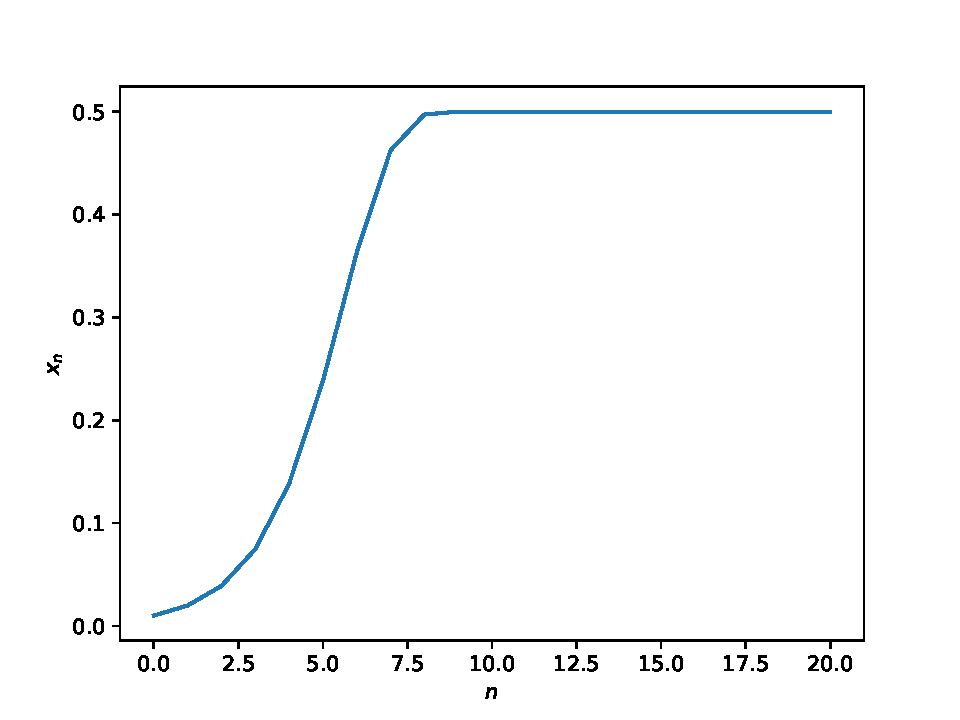
\includegraphics[scale = 0.6]{../figs/first20.pdf}
          \caption{First 20 steps of the discrete logistic equation}
          \label{fig:first20}
        \end{figure}
    \end{enumerate}
  \item
    Figure~\ref{fig:multipleConvergences} shows the evolution of the logistic problem in Eq.~\ref{eq:logit} for various initial conditions.

    \begin{figure}[H]
      \centering
      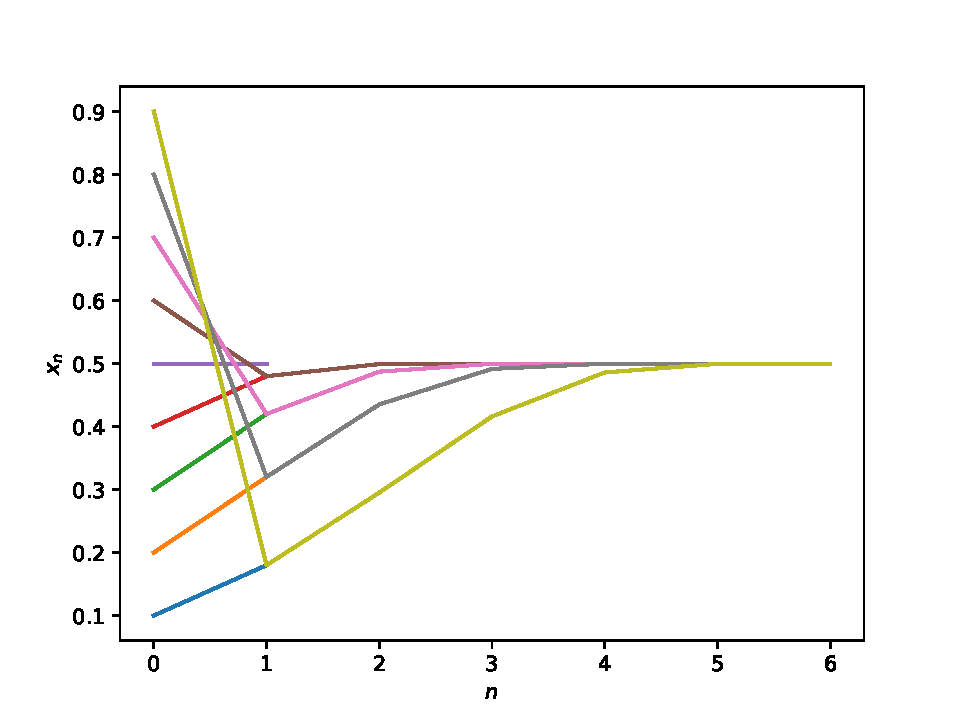
\includegraphics[scale = 0.6]{../figs/multipleConvergences.pdf}
      \caption{Midpoint method solution of a logistic problem}
      \label{fig:multipleConvergences}
    \end{figure}

    All the solutions converge on the value $x = 0.5$.

  \item
    Figure~\ref{fig:equilibriumPoint} shows the logistic equation in Eq.~\ref{eq:logitr} changes as a function of $r$'s value.

    \begin{equation}
      x_{n + 1} = r x_{n} (1 - x_{n}) 
      \label{eq:logitr}
    \end{equation}

    \begin{figure}[H]
      \centering
      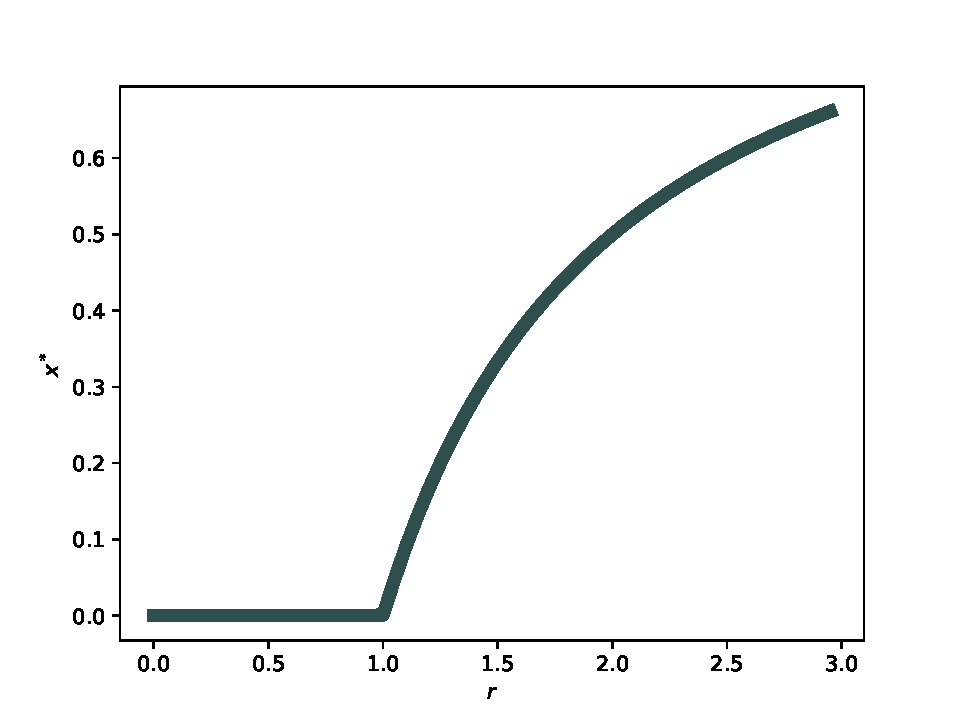
\includegraphics[scale = 0.8]{../figs/equilibriumPoint.pdf}
      \caption{The equilibrium point for various values of $r$}
      \label{fig:equilibriumPoint}
    \end{figure}
  \item
    Figure~\ref{fig:q6} shows the period doubling of the logistic equation.

    \begin{figure}[H]
      \centering
      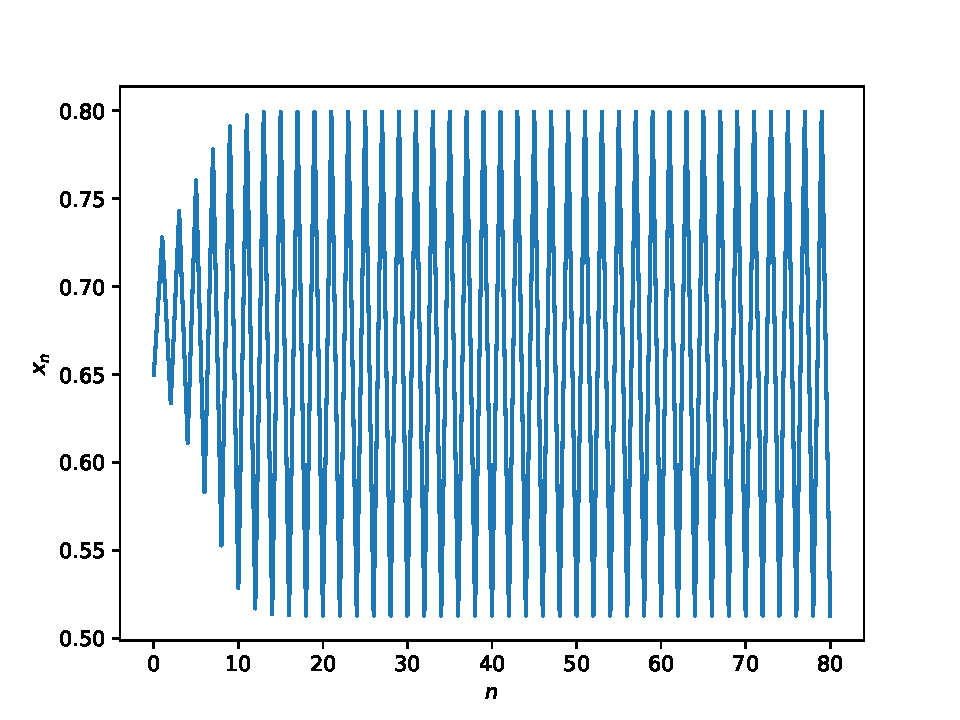
\includegraphics[scale = 0.8]{../figs/q6.pdf}
      \caption{Logistic map Eq.~\ref{eq:logitr} for $r = 3.2$}
      \label{fig:q6}
    \end{figure}
  \item
    Figure~\ref{fig:equilibriumPointsBifurcations} shows a bifurcation in the logistic map.

    \begin{figure}[H]
      \centering
      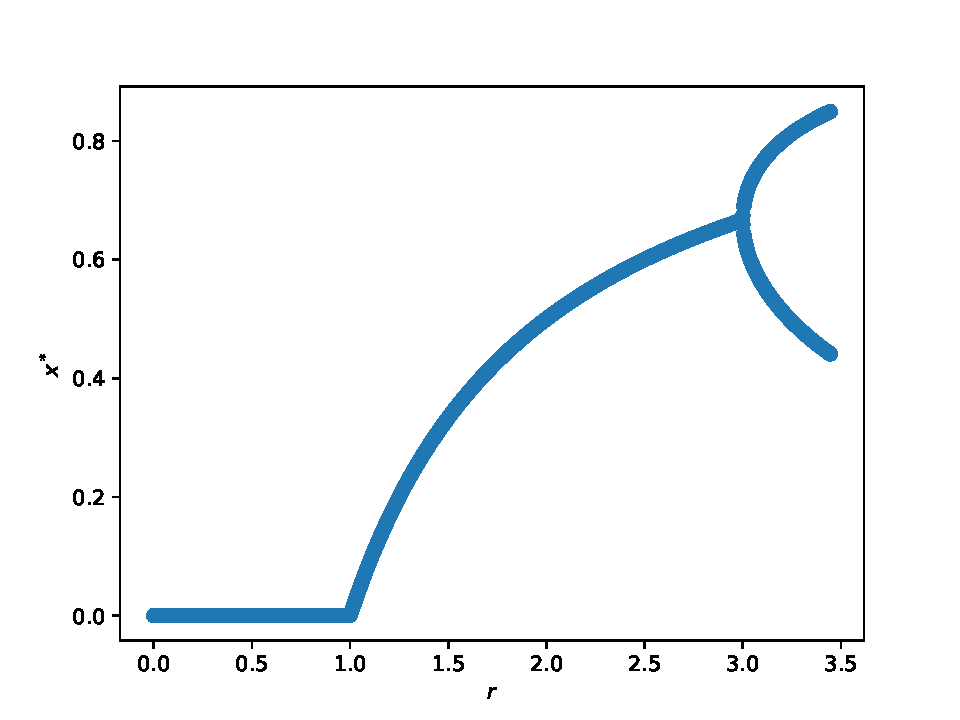
\includegraphics[scale = 0.8]{../figs/equilibriumPointsBifurcations.pdf}
      \caption{Bifurcation in the logistic function}
      \label{fig:equilibriumPointsBifurcations}
    \end{figure}

  \item
    Figure~\ref{fig:furtherEquilibriumPointsBifurcations} shows further bifurcations in the logistic map.

    \begin{figure}[H]
      \centering
      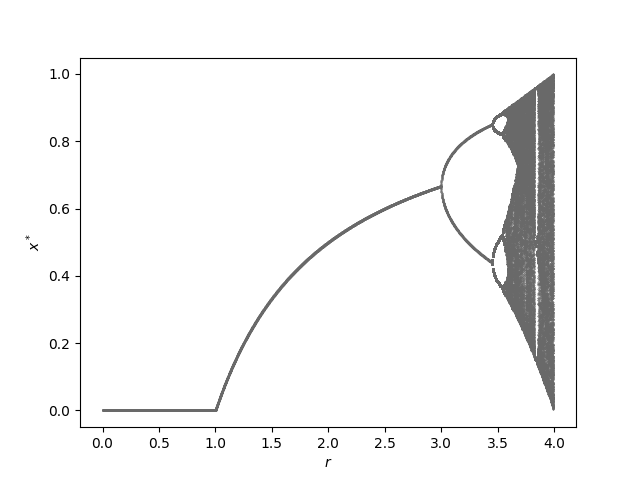
\includegraphics[scale = 0.85]{../figs/furtherEquilibriumPointsBifurcations.png}
      \caption{Bifurcation in the logistic function}
      \label{fig:furtherEquilibriumPointsBifurcations}
    \end{figure}
\end{enumerate}

\end{document}
